% ============================================================
% Backup
% ============================================================
\begin{frame}[t]
\ft{Backup: why the RKKY sign follows the sublattice}\par
\vspace{0.5cm}
\centering
Split the non-local DoS by parity in energy:\quad
$\rho(\vec r,\omega)=\rho_s(\vec r,\omega)+\rho_a(\vec r,\omega),\qquad \rho_{s/a}(-\omega)=\pm\,\rho_{s/a}(\omega)$\par
\vspace{0.3cm}
{\setlength{\fboxsep}{1.5pt}$\displaystyle J_{\rm RKKY}=-2J^2\int_0^W\!\frac{d\Omega_1}{\pi}\int_0^W\!\frac{d\Omega_2}{\pi}\;
\frac{\colorbox{cFM!30}{$\rho_s(\Omega_1)\,\rho_s(\Omega_2)$}\;-\;\colorbox{cAFM!25}{$\rho_a(\Omega_1)\,\rho_a(\Omega_2)$}}{\Omega_1+\Omega_2}$}\par
\vspace{0.1cm}
{\tiny\color{citegray} one loop, particle-hole symmetric band; energies measured from $E_F$; the denominator is positive\par}
\vspace{0.35cm}
\begin{columns}[T]
\begin{column}{0.47\textwidth}
\centering
% sketch: a non-local DoS that is even in energy
\begin{tikzpicture}[x=1cm,y=1cm,font=\scriptsize]
 \draw[->,mygraydark,>=stealth] (-1.9,0)--(1.9,0) node[right] {$\omega$};
 \draw[mygray,dashed] (0,-0.75)--(0,0.95) node[above,mygraydark] {$E_F$};
 \draw[cFM,very thick,domain=-1.7:1.7,samples=60,smooth] plot (\x,{0.75*cos(deg(2.6*\x))*exp(-0.25*\x*\x)});
\end{tikzpicture}\\[3pt]
\colorbox{cFM!30}{\mystrut same sublattice}\\[3pt]
$\rho_s$ dominates: $J_{\rm RKKY}<0$, ferromagnetic\par
\end{column}
\begin{column}{0.47\textwidth}
\centering
% sketch: a non-local DoS that is odd in energy
\begin{tikzpicture}[x=1cm,y=1cm,font=\scriptsize]
 \draw[->,mygraydark,>=stealth] (-1.9,0)--(1.9,0) node[right] {$\omega$};
 \draw[mygray,dashed] (0,-0.75)--(0,0.95) node[above,mygraydark] {$E_F$};
 \draw[cAFM,very thick,domain=-1.7:1.7,samples=60,smooth] plot (\x,{0.75*sin(deg(2.6*\x))*exp(-0.25*\x*\x)});
\end{tikzpicture}\\[3pt]
\colorbox{cAFM!25}{\mystrut opposite sublattice}\\[3pt]
$\rho_a$ dominates: $J_{\rm RKKY}>0$, antiferromagnetic\par
\end{column}
\end{columns}
\vspace{0.3cm}
{\tiny\color{citegray} Curves: sketches of $\rho(\vec r,\omega)$, even and odd in $\omega$. \ Saremi, PRB 76, 184430 (2007)\par}
\end{frame}
% Notes: Eqs. (19)-(21) and App. D of the draft. RKKY couples states below E_F to states above it. Folding both energies onto (0, W) leaves a positive denominator, so the sign is decided by the numerator alone.
% Notes: Even part of the non-local DoS: the product is positive, J_RKKY < 0, ferromagnetic. Odd part: the opposite sign, antiferromagnetic.
% Notes: On a bipartite lattice the same-sublattice non-local DoS is even in energy and the opposite-sublattice one is odd: Saremi's rule. A sufficient condition, not a necessary one.
% Notes: BLG is not exactly particle-hole symmetric (gamma4, Delta'), but the asymmetry is weak and does not change the sign structure.
% Notes: The two curves are sketches, not data.

\begin{frame}[t]
\ft{Backup: A1--B2, screening scale against distance}
\vspace{0.3cm}
\begin{columns}[c]
\begin{column}{0.62\textwidth}
\centering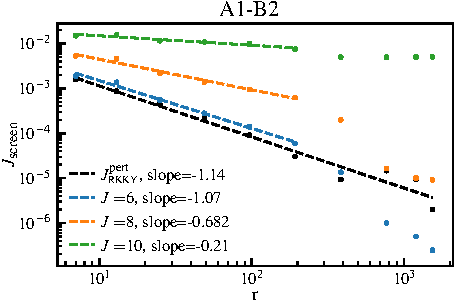
\includegraphics[width=\linewidth]{figures/JvsrSiteAFM.pdf}\par
{\tiny\color{citegray} $J_{\rm screen}$ from the peak of the spin susceptibility\par}
\end{column}
\begin{column}{0.36\textwidth}
{\small\setlength{\tabcolsep}{4pt}
\begin{tabular}{@{}l l@{}}
 coupling & slope\\ \hline
 perturbative & $-1.14$\\
 $J=6$ & $-1.07$\\
 $J=8$ & $-0.68$\\
 $J=10$ & $-0.21$
\end{tabular}\par}
\vspace{0.4cm}
{\small Intermediate $J$: RKKY at short distance, single-impurity Kondo further out\par}
\end{column}
\end{columns}
\end{frame}
% Notes: Weak coupling: perturbative, algebraic decay of the RKKY scale. Very strong coupling: already near the dilute Kondo limit at the shortest distance, almost no distance dependence.
% Notes: Intermediate coupling interpolates: at short distance the impurities still compete through RKKY; further out the perturbative scale is so small that the single-impurity Kondo scale takes over (the points that leave the dashed lines).

\begin{frame}[t]
\ft{Backup: AFM singlet or Kondo? The shape of the entropy}
\vspace{0.5cm}
\begin{columns}[c]
\begin{column}{0.53\textwidth}
\centering
{\small $H=J_{\rm RKKY}\,\vec S_1\cdot\vec S_2,\qquad u=e^{|J_{\rm RKKY}|/T}$\par}
\vspace{0.45cm}
{\small\begin{tabular}{@{}l@{\ \ }l@{}}
 \colorbox{cAFM!25}{\mystrut AFM} & $S=\ln(u+3)-\dfrac{u\ln u}{u+3}$\\[12pt]
 \colorbox{cKondo!20}{\mystrut Kondo} & $S\simeq 2\times\dfrac{\ln 2}{1+T_K/T}$\\[12pt]
 \colorbox{cFM!30}{\mystrut FM} & $S=\ln(1+3u)-\dfrac{3u\ln u}{1+3u}\ \to\ \ln 3$
\end{tabular}\par}
\end{column}
\begin{column}{0.45\textwidth}
\centering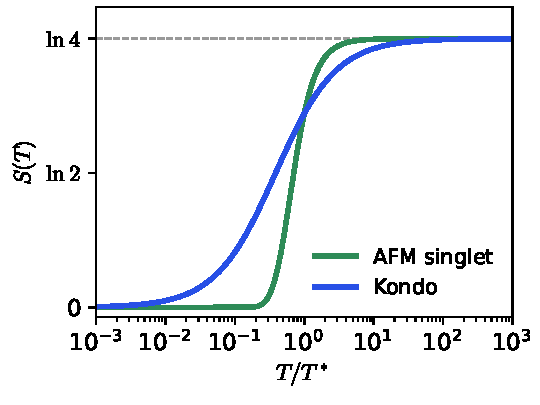
\includegraphics[width=\linewidth]{figures/twospin_entropy.pdf}\par
{\tiny\color{citegray} Both from $\ln 4$ to 0; $T^*$ defined by $S(T^*)=1$\par}
\end{column}
\end{columns}
\vspace{0.5cm}
\centering
\begin{tabular}{@{}l@{\ \ }l@{}}
 \colorbox{cAFM!25}{\mystrut AFM singlet}: & a gap, $S\sim e^{-J_{\rm RKKY}/T}$, gone within one decade\\[3pt]
 \colorbox{cKondo!20}{\mystrut Kondo}: & no gap, $S\sim T/T_K$, spread over several decades
\end{tabular}\par
\end{frame}
% Notes: Both the AFM singlet and Kondo screening take two spins from ln 4 to 0. The shape tells them apart.
% Notes: AFM: two isolated spins with a singlet-triplet gap J_RKKY. The entropy is activated, exp(-J/T): a sharp step, about one decade wide.
% Notes: Kondo: a many-body crossover with no gap. The entropy falls linearly in T (Fermi liquid) and the crossover extends over several decades.
% Notes: These are the dashed curves in the side panels of the A1-B2 slide: weak J follows the AFM form, strong J the Kondo form. Appendix B of the draft; at T = |J|: S = 1.268 (AFM), 1.389 (FM).
% Notes: Figure: figures/make_twospin_entropy.py.

\begin{frame}
\ft{Backup: toy model, RKKY develops a logarithmic decay}
\centering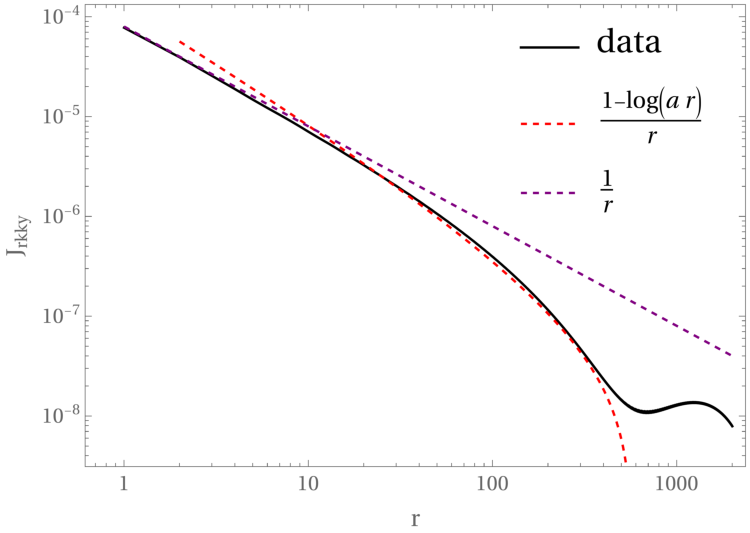
\includegraphics[width=0.6\linewidth]{figures/cosmodel_jrkky.pdf}
\end{frame}
% Notes: - Fig 13: toy model with a vHs: 1/r Fermi-liquid result becomes log(a r)/r behaviour.

